\newpage
\begin{chapterbox}
	\chapter{Theoretical analysis of timescales in turbulent iron combustion} \label{ch:chap3}
\end{chapterbox}
\thispagestyle{empty}
\vfill
\begin{courtesybox}
	Parts of this chapter are published in: \\
	Background image: ...
\end{courtesybox}
\AddToShipoutPictureBG*{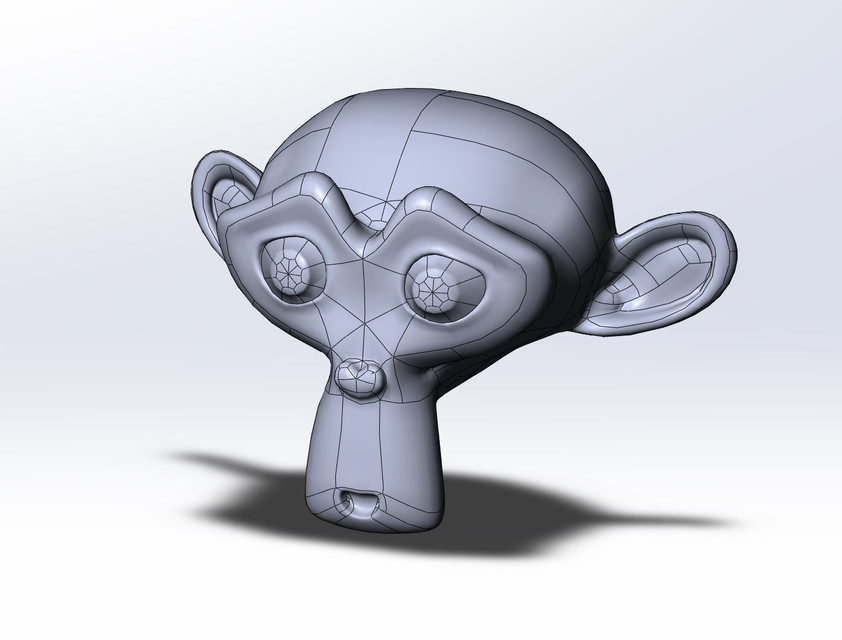
\includegraphics[height=\paperheight,trim=8cm 0 0 0cm]{Figures/chapterCovers/placeholder.jpg}}

\newpage
\thispagestyle{abstract}
\begin{abstractbox}
\section*{Abstract}
\lipsum[1-1]
\end{abstractbox}
\newpage
\section{Introduction}
...

\subsection{Motivations and goals}

\section{Timescales of iron particle clustering}

\subsection{Cluster formation}

\subsection{Cluster evolution}

\section{Timescales of iron particle combustion}

\subsection{Ignition}

\subsection{Oxidation}

\section{Comparison of timescales}

\subsection{Regime map of turbulent iron combustion}

\subsection{Example cases}

\section{Summary}